\documentclass{standalone}
\usepackage{tikz}
\usetikzlibrary{patterns}
\usepackage{pgfplots}
\begin{document}
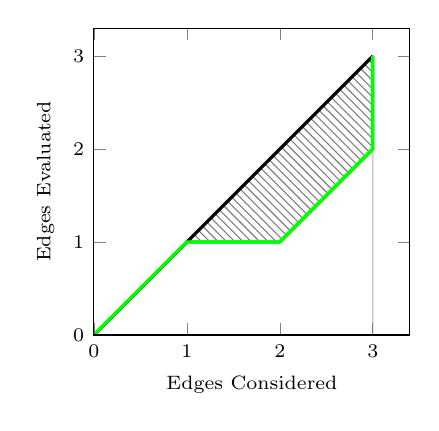
\begin{tikzpicture}[font=\scriptsize]
\begin{axis}[
   xlabel={Edges Considered},
   ylabel={Edges Evaluated},
   %legend pos= north west,
   axis equal image,
   width=2.5in,
   %xmin=0, xmax=5000, ymin=0,
   xmin=0, xmax=3.4, ymin=0,
   %scaled ticks=base 10:-3,
   xlabel near ticks,
   ylabel near ticks,
   axis on top,
   %reverse legend
   ]

% y=x line
\addplot[mark=none,black!20,forget plot] plot coordinates {
   (0,0)
   (3,3)
};

% vertical at first 8 pairs found
\addplot[mark=none,black!20,forget plot] plot coordinates {
   (3,0)
   (3,3)
};

\addplot[mark=none,fill=green!20,pattern=north west lines,pattern color=black!50, draw=black!50,area legend] plot coordinates {
   (0,0)
   (3,3)
} \closedcycle;
%\addlegendentry{Colored Queue}
\addplot[mark=none,fill=white,white,forget plot] plot coordinates {
   (0,0)
   (1,1)
   (2,1)
   (3,2)
   (3,3)
} \closedcycle;

\addplot[mark=none,black!20,forget plot] plot coordinates {
   (3,0)
   (3,2)
};

\addplot[mark=none,green,very thick] plot coordinates {
   (0,0)
   (1,1)
   (2,1)
   (3,2)
   (3,3)
};

\addplot[mark=none,black,very thick] plot coordinates {
   (0,0)
   (3,3)
};

\addplot[mark=none,green,very thick,forget plot] plot coordinates {
   (0,0)
   (1,1)
   (2,1)
   (3,2)
   (3,3)
};

\end{axis}
\end{tikzpicture}%
\end{document}
